%----------------------------------------------------------------------------------------

% Formatvorlage für Arbeiten von Mathias Weigert (Grundlage der Datei und allg. Struktur
% von Micha Schöneberger)

%--------------------------------------VERSION-------------------------------------------

% Version V0.10 - Erstellt von Mathias Weigert am 08.01.2014
%									Basis war die LaTex Dokumente der ZHAW
% Version V0.80 - Erstellt von Mathias Weigert am 24.08.2015
%									Versionsprung, damit Hauptdokument und Configurationsfiles nun selbe
%									Version besitzen. Alle benötigten Files sind nun in Unterverzeichnisse
%									ausgelagert.

% ---------------------------------LADEN DER META DATEN-----------------------------------

% Informationen über das Dokument, wie z.B. Titel, Autor, Jahr etc. werden in der
% Datei _Meta.tex definiert und können danach global verwendet werden.

%----------------------------------------------------------------------------------------

% Formatvorlage für Arbeiten von Mathias Weigert (Grundlage der Datei und allg. Struktur
% von Micha Schöneberger)

%--------------------------------------VERSION-------------------------------------------

% Version V0.75 - Erstellt von Mathias Weigert am 16.09.2013
%				  Bisher ungenützten "Balast" entfernt und zweite Matrikelnummer
%				  eingefügt.

%----------------------------------- INFORMATIONEN ---------------------------------------

% 	Definition von globalen Parametern, die im gesamten Dokument verwendet
% 	werden können (z.B auf dem Deckblatt etc.).
%-----------------------------------------------------------------------------------------

\newcommand{\titel}{Collector}	            % Titel des Dokumentes
\newcommand{\untertitel}{Semesterarbeit}	% Untertitel des Dokumentes
\newcommand{\autorFirst}{Mathias Weigert}	% Autor
\newcommand{\jahr}{2015}					% Jahr der Arbeit

\newcommand{\version}{Kick Off Semesterarbeit}				% Dokument Version
\newcommand{\gueltig}{2015}				    % Dokument Gültigkeit
\newcommand{\initial}{mwe}					% Initial des Autors
\newcommand{\freigabe}{}					% Freigegeben durch

\newcommand{\path}{D:\textbackslash Data\textbackslash Studium\textbackslash WorkSpace\textbackslash Collector\textbackslash Protokoll\textbackslash}	% Pfad des Files
\newcommand{\file}{KickOff.pdf}    	       % Name des Files

%-----------------------------------------------------------------------------------------

% ----------------------------------------------------------------------------------------

% ----------------------------------DOKUMENTENKOPF----------------------------------------

% Diese Vorlage basiert auf "scrreprt" aus dem koma-script.
% Die Option "draft" sollte beim fertigen Dokument ausgeschaltet werden.

\documentclass[
	11pt,				% Schriftgröße
	ngerman,			% für Umlaute, Silbentrennung etc.
	a4paper,       		% Papierformat
	oneside,			% einseitiges Dokument
	titlepage,			% es wird eine Titelseite verwendet
	final				% Status des Dokuments (final/draft)
]{scrbook}				% KOMA Script-Klassen: scrbook, scrreprt, scrartcl, scrlttr2.
						% Die Angabe einer Dokumentenklasse ist obligatorisch.

% ----------------------------------------------------------------------------------------

% -----------------------------PACKAGES EINLESEN------------------------------------------
% Weitere Packages, die benötigt werden, sind in die Datei Packages.tex "ausgelagert", um
% die Vorlage möglichst Übersichtlich zu halten.

%----------------------------------------------------------------------------------------

% Formatvorlage fuer Arbeiten von Mathias Weigert (Grundlage der Datei und allg. Struktur
% von Micha Schoeneberger)

%--------------------------------------VERSION-------------------------------------------

% Version V0.75 - Erstellt von Mathias Weigert am 16.09.2013
%				          Etwas aufgeraeumt, muss mal bei Zeit detailiert Ueberarbeitet werden.
%         V0.80 - Erstellt von Mathias Weigert am 24.08.2015
%                 Kleinere Anpassungen und nochmalieges "aufräumen" der einzelnen
%                 Packages.

%---------------------------------- INFORMATIONEN ---------------------------------------

% 	Definition von globalen Parametern, die im gesamten Dokument verwendet
% 	werden koennen (z.B auf dem Deckblatt etc.).
%----------------------------------------------------------------------------------------

\usepackage{cite}					% Verbesserte Zitierungsmoeglichkeiten
\usepackage{tocbasic}

%----------------------- FORMATIERUNG KOPF- UND FUSSZEILE -------------------------------

\usepackage
[automark,							% Automatische Kopfzeile
%headtopline,						% Linie ueber dem Seitenkopf
%plainheadtopline,					% Plain, Linie ueber dem Seitenkopf
headsepline,						% Linie zwischen Kopf und Textkoerper
ilines,								% Trennlinie linksbuendig ausrichten
%plainheadsepline,					% Plain, Linie zwischen Kopf und Textkoerper
footsepline,						% Linie zwischen Textkoerper und Fuss
plainfootsepline,   				% Plain, Linie zwischen Textkoerper und Fuss
%footbotline,						% Linie unter dem Fuss
%plainfootbotline   				% Plain, Linie unter dem Fuss
]{scrpage2}

%----------------------------------------------------------------------------------------


%-------------------------- ANPASSUNG LANDESSPRACHE--------------------------------------

\usepackage{ngerman}

%----------------------------------------------------------------------------------------


%--------------------------------- UMLAUTE-----------------------------------------------

\usepackage[T1]{fontenc}			% Dadurch ist auch sichergestellt, dass in einem PDF
									% Umlaute gefunden werden.
%\usepackage[utf8x]{luainputenc}
\usepackage[utf8]{inputenc}			% Unterstützung erweiterter Zeichensätze mit
									%  unterschiedlichen Kodierungen
									% (z. B. ae, oe,  usw.)
\usepackage{textcomp} 				% Text Companion Schriften (grosse Symbolbibliothek)

%----------------------------------------------------------------------------------------

\usepackage{pifont}					% PostScript standard Symbol and Dingbats fonts

%--------------------------------EIGENE REFERENZIERUNG-----------------------------------

\newcommand{\refTC}[1]{ \ref{#1} \nameref{#1}  }
% gibt aus z.B.: 1.1.3 Erwartetes Resultat (<Kapitelnummer> <Kapitelname>)

%----------------------------------------------------------------------------------------


%----------------------------------- GRAFIKEN--------------------------------------------

\usepackage[dvips,final]{graphicx}		% Einbinden von EPS-Grafiken [draft oder final]
\graphicspath{{pic/}} 					% Hier liegen die Bilder des Dokuments

%----------------------------------------------------------------------------------------

\usepackage{amsmath,amsfonts}			% Befehle aus AMSTeX fuer mathematische Symbole
										% z.B. \boldsymbol \mathbb
\usepackage{multirow}					% Packages fuer Tabellen

%-------------------------------- OWN COLORS---------------------------------------------

\usepackage{conf/rgbcolor}				% Eigene Farbdefinitionen nach RGB Chart
\usepackage[table]{xcolor}				% Um Tabellen einzuf�rben

%----------------------------------------------------------------------------------------

\usepackage{makeidx}					% Fuer Index-Ausgabe; \printindex

%------------------------------ QUELLCODE AUSGABE----------------------------------------

%************************************************************************************
%*                                                    Definitionen zur Quellcode Darstellung                                                   *
%************************************************************************************

\usepackage{listings}

\lstset {language=C++,
	keywordstyle={\color{Blue}\bfseries},
	commentstyle={\color{ForestGreen}\slshape},
	stringstyle={\color{Purple}},
	backgroundcolor={\color{PowderBlue}},
	showstringspaces=fales,
	stepnumber=2,
	numbers=left,
	numberstyle=\tiny}

\lstset {language=SQL,
	keywordstyle={\color{IndianRed}\bfseries},
	commentstyle={\color{ForestGreen}\slshape},
	identifierstyle=\ttfamily\color{CadetBlue}\bfseries,
	stringstyle={\color{Purple}},
	backgroundcolor={\color{Tan}},
	showstringspaces=fales,
	stepnumber=2,
	numbers=left,
	numberstyle=\tiny}						% Eigene Ausgabeformatierungen fuer Quellcode

%----------------------------------------------------------------------------------------


%-------------------------- ZEILENABSTAENDE UND SEITENRAENDER------------------------------

\usepackage{setspace}					% hat zur Benützung 3 Optionen: [singlespacing,
										% onehalfspacing, doublespacing]
\usepackage{geometry}
\usepackage{lineno}						% ermoeglicht das Numerieren der Zeilen

\usepackage{titlesec}
\titleformat{\chapter}
{\normalfont\huge\bfseries}{\thechapter.}{11pt}{\Huge}
\titlespacing*{\chapter}{0pt}{-40pt}{15pt}


% Symbolverzeichnis --------------------------------------------------------
% Symbolverzeichnisse bequem erstellen, beruht auf MakeIndex.
% makeindex.exe %Name%.nlo -s nomencl.ist -o %Name%.nls
% erzeugt dann das Verzeichnis. Dieser Befehl kann z.B. im TeXnicCenter
% als Postprozessor eingetragen werden, damit er nicht staendig manuell
% ausgefuehrt werden muss.
% Die Definitionen sind ausgegliedert in die Datei Abkuerzungen.tex.
% --------------------------------------------------------------------------
\usepackage[intoc]{nomencl}
  \let\abbrev\nomenclature
  \renewcommand{\nomname}{Abkürzungsverzeichnis}
  \setlength{\nomlabelwidth}{.25\hsize}
  \renewcommand{\nomlabel}[1]{#1 \dotfill}
  \setlength{\nomitemsep}{-\parsep}


%inserted november 2012 / Micha
\usepackage[normalem]{ulem}
\newcommand{\markup}[1]{\uline{#1}}


\usepackage{floatflt}							% Zum Umfliessen von Bildern

\usepackage[hyphens]{url}			% bricht lange URL's um, ohne dass der Link defekt ist
%\usepackage{url}

%-------------------------------PDF OPTIONEN----------------------------------------------

\usepackage[
bookmarks,
bookmarksopen=true,
pdftitle={\titel},
pdfauthor={\autorFirst},
pdfcreator={\autorFirst},
pdfsubject={\titel},
pdfkeywords={\titel},
colorlinks=true,
linkcolor=red, 							% einfache interne Verknuepfungen
anchorcolor=black,						% Ankertext
citecolor=blue, 						% Verweise auf Literaturverzeichniseintraege im Text
filecolor=magenta, 						% Verknuepfungen, die lokale Dateien oeffnen
menucolor=red, 							% Acrobat-Menuepunkte
urlcolor=cyan,
%linkcolor=black, 						% einffdrtext
%citecolor=black, 						% Verweise auf Literaturverzeichniseintraege im Text
%filecolor=black, 						% Verknuepfungen, die lokale Dateien öffnen
%menucolor=black,						% Acrobat-Menuepunkte
%urlcolor=black,
backref,
%pagebackref,
plainpages=false,						% zur korrekten Erstellung der Bookmarks
pdfpagelabels,							% zur korrekten Erstellung der Bookmarks
hypertexnames=false,					% zur korrekten Erstellung der Bookmarks
linktocpage 							% Seitenzahlen anstatt Text im Inhaltsverzeichnis verlinken
]{hyperref}

\usepackage[final]{pdfpages}			%Ermoeglicht andere PDF ins Dokument einzufuegen.

%-----------------------------------------------------------------------------------------

\usepackage{chngcntr}					% Zum fortlaufenden Durchnummerieren der Fussnoten

% fuer lange Tabellen
\usepackage{longtable}
\usepackage{array}
\usepackage{ragged2e}
\usepackage{lscape}

%Spaltendefinition rechtsbaendig mit definierter Breite
\newcolumntype{w}[1]{>{\raggedleft\hspace{0pt}}p{#1}}

% Formatierung von Listen aendern
\usepackage{paralist}
% \setdefaultleftmargin{2.5em}{2.2em}{1.87em}{1.7em}{1em}{1em}

\usepackage{lastpage}				% Dient zum ermitteln der Seiten eines Dokuments
	% lade ausgelagerte Packages

% ----------------------------------------------------------------------------------------

% -----------------------KOPF- UND FUSSZEILE, SEITENRÄNDER...-----------------------------
% Diese Einstellungen sind im Dokument Seitenstil ausgelagert.

% --------------------------------------------------------------------------ZEILENABSTAND-------------------------------------------------------------------------------------------

\onehalfspacing								% setzte den Zeilenabstand / Möglichkeiten: singlespacing, onehalfspacing, doublespacing

%------------------------------------------------------------------------------------------------------------------------------------------------------------------------------------------

			
% -------------------------------------------------------------------------SEITENRÄNDER--------------------------------------------------------------------------------------------

\geometry{									% definiert Papierformat und die Ränder
paper=a4paper,left=35mm,right=25mm,top=10mm, bottom=48mm
}

%------------------------------------------------------------------------------------------------------------------------------------------------------------------------------------------


% ------------------------------------------------------------------------KOPF- UND FUSSZEILE--------------------------------------------------------------------------------------

\pagestyle{scrheadings}							%
\renewcommand*{\chapterpagestyle}{scrheadings}			% Kopf- und Fußzeile auch auf Kapitelanfangsseiten


\renewcommand{\headfont}{\normalfont}				% definiert die Schriftart für die Kopfzeile (z.B: auch möglich: \sffamily)

% Kopfzeile ----------------------------------------------------------------
%\ihead{\large{\textsc{\titel}}\\[1ex] \textit{\headmark}}
\ihead{\textit{\headmark}}
\chead{\qquad \qquad \qquad \qquad \qquad \qquad \qquad \quad \qquad \qquad \qquad \qquad \qquad \qquad \qquad   
\includegraphics[scale=0.08]{pic/ZHAW_logo.png}}%\ohead{
\includegraphics[scale=0.08]{ZHAW_logo.png}} % setze Aussenseite der Kopfzeile
\setlength{\headheight}{30mm} 						% Höhe der Kopfzeile
\setheadwidth[0pt]{textwithmarginpar} 				% Kopfzeile über den Text hinaus verbreitern
\setheadsepline[text]{0.4pt} 						% Trennlinie unter Kopfzeile

\ifoot{\autorFirst}								% setze Innenseite der Fusszeile	
\cfoot{}									% setze Center-Fusszeile
\ofoot{\pagemark}								% setze Aussenseite Fusszeile
\setfootsepline[text]{0.4pt} 						% Trennlinie über Fusszeile

%------------------------------------------------------------------------------------------------------------------------------------------------------------------------------------------
%  INFO:

%  @\pagemark								% Kapitelname
%  @ihead									% Mit dieser Angabe wird die Innenseite ("i" = "inside") des Seitenkopfs definiert
%  @chead									% Mit dieser Angabe wird die Mitte ("c" = "center") des Seitenkopfs definiert
%  @ohead									% Mit dieser Angabe wird die Außenseite ("o" = "outside") des Seitenkopfs definiert
%  @ifoot									% Mit dieser Angabe wird die Innenseite des Fusszeile definiert
%  @cfoot									% Mit dieser Angabe wird die Mitte des Fusszeile definiert
%  @ofoot									% Mit dieser Angabe wird die Aussenseite des Fusszeile definiert

% siehe auch: http://www.jochen-lipps.de/latex/kopfzeile.php
% siehe auch: http://www2.informatik.hu-berlin.de/~piefel/LaTeX-PS/Archive-2004/V07-footnote.pdf
%------------------------------------------------------------------------------------------------------------------------------------------------------------------------------------------


% --------------------------------------------------------SCHUSTERJUNGEN UND HURENKINDER----------------------------------------------------------------------------------

\clubpenalty = 10000							% Disable single lines at the start of a paragraph (Schusterjungen)
\widowpenalty = 10000 							% Disable single lines at the end of a paragraph (Hurenkinder)
\displaywidowpenalty = 10000						% Disable single lines at the end of a paragraph (Hurenkinder)

%------------------------------------------------------------------------------------------------------------------------------------------------------------------------------------------

% -----------------------------------------------------------AUSGABE QUELLCODE FORMATIEREN---------------------------------------------------------------------------------

\lstset{numbers=left, numberstyle=\tiny, numbersep=5pt, breaklines=true}
\lstset{emph={square}, emphstyle=\color{red}, emph={[2]root,base}, emphstyle={[2]\color{blue}}}									%------------------------------------------------------------------------------------------------------------------------------------------------------------------------------------------

\frenchspacing								% erzeugt ein wenig mehr Platz hinter einem Punkt
\counterwithout{footnote}{chapter}					% Fußnoten fortlaufend durchnummerieren
	% lade spezifische Kopf- und Fusszeilen

% ----------------------------------------------------------------------------------------

\begin{document}

\setlength{\parindent}{0pt}		% sorgt dafür das es keinen Einzug am Absatzanfang gibt
\setcounter{secnumdepth}{3}		% legt die Tiefe bei Nummerierung von Überschriften fest
\setcounter{tocdepth}{3}		% legt Schachtelungstiefe bei Inhaltsverzeichnis fest

% ----------------------------------------------------------------------------------------

% ---------------------DECKBLATT, INHALT & VERSIONSVERWALTUNG-----------------------------

%----------------------------------------------------------------------------------------

% Formatvorlage für Arbeiten von Mathias Weigert (Grundlage der Datei und allg. Struktur
% von Micha Schöneberger)

%--------------------------------------VERSION-------------------------------------------

% Version V0.75 - Erstellt von Mathias Weigert am 16.09.2013
%				  				Der besseren Übersicht wegen Informationen aus zwei Seiten verteilt
% 				V0.80 - Erstellt von Mathias Weigert am 24.08.2015
%									Deckblatt auf einer Seite mit etwas weniger Information. Die Zukunft
%									wird so aussehen, dass ich verschiedene Deckblätter erstelle welche
%									nach Bedarf ins Dokument eingebunden werden.

%------------------------------------SEITENLAYOUT-----------------------------------------

% Informationen Über das Dokument, wie z.B. Titel, Autor, Matrikelnr. etc werden in der
% Datei _Meta.tex definiert und können danach global verwendet werden.

%\thispagestyle{empty} 		% Dokument ohne Kopfzeile und ohne Seitennummerierung.
\thispagestyle{plain} 		% Mit Seitennummerierung (Standard)
%\thispagestyle{headings} 	% Generiert eine automatische Kopfzeile mit Seitenzahl und
							% Zwischenüberschriften
%\thispagestyle{myheadings} % Erlaubt die Erstellung eigener Kopf- und Fußzeilen
%\thispagestyle{fancy} 		% Erlaubt die Verwendung der in dem Paket "fancyhdr"
							% definierten Befehle zur Erstellung eigener Kopf- und
							% Fußzeilen

%-----------------------------------------------------------------------------------------

%----------------------------------SETZE TITELBLATT---------------------------------------

\begin{titlepage}

\begin{center}

\includegraphics[scale=0.25]{pic/ZHAW_Titel}			% binde die Grafik ein
\\[12ex]
\huge{\textbf{\textsc{\titel}}}							% setze Schriftgrösse für Titel
\\[1.5ex]
\LARGE{\textbf{\untertitel}}							% setze Schriftgrösse für Untertitel
\\[6ex]
\normalsize												% setze Schriftgrösse zurück auf Normalschrift

\begin{tabular}{w{3cm}p{6cm}}
\\[12ex]Autor: & \quad \autorFirst						% Angabe des Studienbereichs
\end{tabular}
\\[24ex]
\copyright\ \jahr\\
\end{center}

\singlespacing											% einfacher Zeilenabstand
\small													% setze kleine Schrift
\noindent												%	Sorgt am Anfang eines Absatzes dafür, daß die
														% erste Zeile nicht eingerückt wird.


%----------------------------GNU FREE DOCUMENTATION LICENSE---------------------------------
Es wird die Erlaubnis gegeben dieses Dokument zu kopieren, verteilen und/oder zu verändern
unter den Bedingungen der GNU Free Documentation License, Version 1.3 oder einer späteren, von
der Free Software Foundation veröffentlichten Version; mit den Unveränderlichen Abschnitten
DEREN TITEL	AUFGEZÄHLT sind, mit den Vorderseitentexten die AUFGEZÄHLT sind, und mit den
Rückseitentexten die AUFGEZÄHLT sind. Eine Kopie dieser Lizenz ist in	dem Abschnitt enthalten,
der mit \href{http://www.gnu.org/copyleft/fdl.html}{GNU Free Documentation License} betitelt ist.

%--------------------------------------COPYRIGHT-------------------------------------------
%Dieses Werk einschließlich seiner Teile ist \textbf{urheberrechtlich geschützt}. Jede
%Verwertung außerhalb der engen Grenzen des Urheberrechtsgesetzes ist ohne Zustimmung des
%Autors unzulässig und strafbar. Das gilt insbesondere für Vervielfältigungen, Übersetzungen,
%Mikroverfilmungen sowie die Einspeicherung und Verarbeitung in elektronischen Systemen.

\end{titlepage}
		% Deckblatt

\tableofcontents				% Inhaltsverzeichnis

\chapter*{Version}

Angabe der aktuellen Version des Dokuments. Alle Änderungen, werden mit Versionsnummer, Datum, Autor und Informationen betreffend der Änderung dokumentiert.\\

\begin{tabular}{|c|l|c|l|}
	\rowcolor{black} {\color{white}\textbf{Version}} & {\color{white}\textbf{Datum}} & {\color{white}\textbf{Autor}} & {\color{white}\textbf{Bemerkung}} \\
	0.01 & 30.11.15 & M. Weigert & Initiales Dokument \\ \hline
	\rowcolor{DarkSeaGreen} 0.02 & 30.11.15 & M. Weigert & Aufgabe hinzugefügt \\ \hline
	0.03 & 02.12.15 & M. Weigert & Neue LaTex Konfiguration, Literaturverzeichnis, erste Recherche \\ \hline
	\rowcolor{DarkSeaGreen} 0.04 & 04.12.15 & M. Weigert & Kapitelstruktur angelegt. Recherche fortgeführt \\ \hline
	0.04 & 03.02.16 & M. Weigert & Zeitmanagement und Feinstruktur \\ \hline
	\rowcolor{DarkSeaGreen} 0.05 & 06.02.16 & M. Weigert & Neue Datenstruktur und Anforderungen dokumentiert. \\ \hline
\end{tabular}

\chapter*{Zeitmanagement}

\begin{tabular}{|c|l|c|c|l|}
	\rowcolor{black} {\color{white}\textbf{Datum}} & {\color{white}\textbf{Start}} & {\color{white}\textbf{Ende}} & {\color{white}\textbf{Zeit (min.)}} & {\color{white}\textbf{Bemerkung}} \\
	03.02.16 & 20:30 & 21:00 & 30 & Zeitmanagement und Feinplanung (Basis) \\ \hline
	\rowcolor{DarkSeaGreen} 06.02.16 & 11:00 & 12:45 & 105 & Angefangen mit der Anforderungsanalyse \\ \hline
	06.02.16 & 13:30 & & & Weiter an Anforderungsanalyse gearbeitet. \\ \hline
\end{tabular}	% Versionsverwaltung

% ----------------------------------------------------------------------------------------

% -----------------------------INHALT DES DOKUMENTS---------------------------------------

% Hier können jetzt die einzelnen Kapitel implementiert werden. Sie müssen in den
% entsprechenden .TEX-Dateien vorliegen. Die Dateinamen können natürlich angepasst werden.

% ----------------------------------------------------------------------------------------

\chapter{Aufgabe}

\begin{longtable}{rp{12cm}}
	\textbf{Projektname} & Collector \\
	\textbf{Projektstatus} & Die Arbeit ist freigegeben (Eine Semester- oder Bachelorarbeit kann nur durch die Studiengangsleitung freigegeben werden). \\
	\textbf{Projekttyp} & Semesterarbeit \\
	\textbf{Letzter Abgabetermin} & 5. Mai 2016 \\
	\textbf{Zusammenfassung} & Management von Sammlungen im Bereich: Bücher, Filme (DVD \& Blue Ray) und Computer-/Konsolenspielen durch eine Android App. \\
	\textbf{Student} & Mathias Weigert \\
	\textbf{Betreuungsperson} & Michael Reiser \\
	\textbf{Ausgangslage} & Ich besitze (sehr) viele Bücher, Filme und Spiele (Computer \& Konsolen). Seit einiger Zeit passiert es immer häufiger, dass ich auf Flohmärkten und in Brockenhäusern Fehlkäufe tätige und ich beim Einsortieren meiner neuen Schätze feststelle, dass ich dieses spezielle Buch, Film oder Spiel bereits besitze. Vor ein paar Jahren hatte ich eine Software mit Barcodescanner für meinen PC (\href{http://intelliscanner.com/products/media/index.html}{http://intelliscanner.com/products/media/index.html}), welche meine Sammlung auch online zur Verfügung stellte. Als ich versuchte die Datenbank von Windows XP auf Windows 7 zu migrieren, traten einige Probleme auf. Ich machte mich auf die Suche nach Alternativen im Bereich Apps für mein Smartphone, da ich in anderen Bereichen bereits gute Software für die Verwaltung meiner Sammlungen (z.B. Magic the Gathering) gefunden hatte. Bisher konnte ich noch keine App finden, welche all meine Ansprüche vereint. \\
	\textbf{Ziel der Arbeit} & Eine funktionierende App, welche mittels der eingebauten Kamera (als Barcodescanner) das Buch, den Film oder das Spiel identifiziert und einer Sammlung hinzufügt. Die Items der Sammlung sollen vom Benutzer verwaltet werden können. Eine weitere Funktion soll das Verleihen einzelner Items ermöglichen, so dass der User die maximale Kontrolle über seine Sammlung hat. \\
	\textbf{Aufgabenstellung} & \begin{enumerate}
	\item Recherche \newline
		Herausfinden, was es momentan auf dem Markt (Google Play / Amazon App Market) im Bereich der Apps gibt, welche helfen Sammlungen im Bereich Bücher, DVD und
		Konsolen-Spiele zu verwalten. Überblick erstellen über die einzelnen Apps und Ihre Fähigkeiten.
	  \item Ist-Analyse \newline
		Momentan existiert noch keine vergleichbare App. Alle existierenden Apps können nur Teile der geplanten gesamten Funktionalität der Collector App abdecken.
	  \item Anforderungsanalyse \newline
		Collector soll eine App sein, welche für folgende Medientypen: Bücher, DVD und Computer- oder Konsolenspiele den Besitzer beim Verwalten seiner Sammlung unterstützt. Egal welchem Medientyp ein Item angehört, können mit der App folgende Aktionen durchgeführt werden können.
	  \begin{itemize}
		\item Anlegen eines neuen Items
		\item Ausgabe aller Items (inklusive Filterfunktion)
		\item Bearbeiten eines Items
		\item Löschen eines Items
		\item Exportieren aller Items (inklusive Filterfunktion)
		\item Verwalten verliehener Items
		\item Speichern der Items (in einer Datenbank)
	  \end{itemize}
	  \item Konzept \newline
		Um das Anlegen einzelner Items zu erleichtern, soll die App mittels der Kamera den Barcode des Items scannen und einen Abgleich mit verfügbaren Internetdatenbanken in den Bereichen der einzelnen Medientypen durchführen. Fehlende oder fehlerhafte Daten bei einzelnen Items soll der Benutzer manuell eingeben bzw. anpassen können. Die Ausgabe der Items einer Sammlung soll entweder visuell (auf dem Bildschirm) oder per Datenexport (CSV oder XML) erfolgen. Ein Filter, welchen die App zur Verfügung stellt, kann genutzt werden um die Ausgabe der Items einzuschränken. Eine Verleihverwaltung rundet die App ab und hilft dem User nicht den Überlick über verliehene Items seiner Sammlung zu verlieren.
	\end{enumerate} \\
	& \begin{enumerate}
		\setcounter {enumi}{4}
	  \item Prototyp \newline
		  Der Prototyp der App soll alle Funktionen, welche in Punkt 4. definiert wurden, fehlerfrei ausführen können. Die App soll auf möglichst vielen Android Geräten funktionieren.
	  \item Testing \newline
		  Das Testing wird durch das anlegen, möglichst vieler Unterschiedlicher Items aller Medientypen, erfolgen. Die einzelnen Items werden dokumentiert und auftretende Schwierigkeiten beim Anlegen der Items werden ebenfalls dokumentiert. Sobald ein gewisser Grundstock an Items in der Datenbank hinterlegt sind, werden die restlichen Funktionen getestet.
	\end{enumerate} \\
	\textbf{Erwartete Resultate} & \begin{enumerate}
		\item Recherche \newline
			Gründlicher Marktüberblick, welcher die Apps übersichtlich Darstellt, welche ähnliche oder sogar identische Funktionen wie die App Collector besitzen. Nach der kurzen Vorstellung der einzelnen Apps, wird ein Überblick alle recherchierten Apps im Vergleich zu Collector zeigen.
		\item Ist-Analyse \newline
			Es wird anhand der Funktionen von Collector dargestellt, das es keine der existierenden Apps den selben Funktionsumfang haben wie Collector.
		\item Anforderungsanalyse \newline
			Alle beschriebenen Funktionalitäten sollen fehlerfrei in der App umgesetzt werden.
		\item Konzept \newline
			Die eingesetzten Werkzeuge und Konzepte sollen dokumentiert werden. Einzelne für die Funktion der App wichtige Klassen und Funktionen sollen detailliert dargestellt werden. Design-Entscheidungen sollen erklärt werden. 
		\item Prototyp \newline
			Der Prototyp soll mindestens auf dem Test-Smartphone (Samsung Galaxy XCover) fehlerfrei funktionieren.
	\end{enumerate}\\
	& \begin{enumerate}
		\setcounter{enumi}{5}
		\item Testing \newline
			Sowohl die automatisierten als auch die manuellen Tests sollen ausführlich, klar und komplett dokumentiert werden.
	\end{enumerate}
\end{longtable}
\chapter{Recherche}

Die komplette Recherche findet im Google App Store \href{https://play.google.com/store/apps}{GooglePlay} statt. Für die nachfolgende Ist-Analyse werde ich noch auf die einzelne Apps aus dem Apple App Store verweisen, welche ich selbst einsetze und welche mir im Bezug auf Funktionalität und Design von \emph{Collector} die ein oder andere Idee geliefert haben.

\section{My books}

Diese App dient der Inventarisierung und Organisation der persönlichen Bibliothek. Es ist einfach die komplette Bücher Sammlung zu speichern. Bücher können einfach, durch scannen des Barcode hinzugefügt werden.\\

Features:
\begin{itemize}
	\item Hinzufügen eines Buches durch scannen des Barcode
	\item Hinzufügen eines Buches durch eingeben des ISBN Code
	\item Hinzufügen eines Buches durch eingeben von Titel, Autor, etc...
	\item Ansicht aller Bücher eines Autors
	\item Im- und Export aller Daten in ein File
\end{itemize}

Durch eine Vielzahl von Listen kann der Bücher Katalog organisiert werden.
\begin{itemize}
	\item Bücher welche ich kaufen möchte
	\item Bücher welche ich nochmals lesen möchte
	\item Bücher welche mir gefallen haben
	\item Bücher welche ich verliehen habe
\end{itemize} 

Es gibt eine Vielzahl von Filtermöglichkeiten, wie Genre, Autor, Beurteilung, Leser und viele weiteren.
\chapter{Ist-Analyse}

Wie man an Kapitel \ref{ch:recherche} ersehen kann...
\chapter{Anforderungsanalyse}

\section{Funktionen}

Die App Collector soll den folgenden Beschriebenen Funktionsumfang besitzen. Dieser wurde anhand der Recherche, der Ist-Analyse und dem Bedarf von M. Weigert ermittelt. Probleme bei der Umsetzung der Funktionen und deshalb nötige Anpassungen werden im Kapitel \ref{ch:Umsetzung} ab Seite \pageref{ch:Umsetzung} dokumentiert.

\newpage

\begin{landscape}
	\section{Übersicht Funktionen}
	\label{sec:UebersichtFunktion}
	\begin{figure}[htbp]
		\centering
		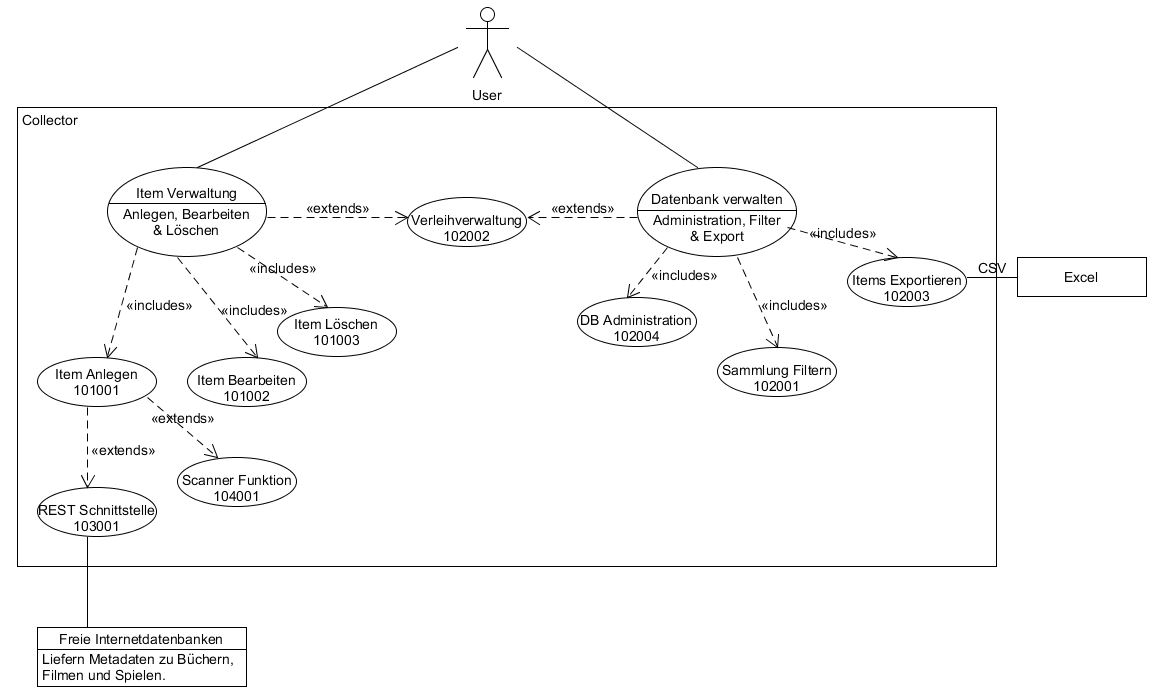
\includegraphics[scale=0.65]{pic/SystemUseCase}
		\caption{Überblick Funktionen}
	\end{figure}
\end{landscape}

\subsection{Anlegen eines Items}

[101001] Funktion: Item Anlegen\\

Das Anlegen eines neuen Items soll auf zweierlei Arten Möglich sein.

\begin{enumerate}
	\item Manuell
	\item Automatisch
\end{enumerate}

Nach der Auswahl {\color{IndianRed}\texttt{Neues Item}} wird standardmässig der Screen für das automatische Anlegen eines Items, mit aktivierter Kamera, geöffnet. Auf diesem Screen gibt es einen Button für das manuelle Anlegen eines Items.

\subsubsection{Manuelles Anlegen eines Items}

Sobald der User {\color{IndianRed}\texttt{manuell}} ausgewählt hat öffnet sich der Screen für Bearbeiten und Manuelles anlegen eines Items. Da es sich hierbei um die neu Anlage eines Items handelt ist der Screen noch komplett ohne angezeigte Daten.\\

Nun kann der User alle Parameter, welche ein Item besitzt manuell eingeben und speichern. Um welche Daten es sich hierbei handelt ist in diesem Kapitel im Absatz \ref{sec:Felder} ab Seite \pageref{sec:Felder} dokumentiert.

\begin{figure}[htbp]
	\centering
	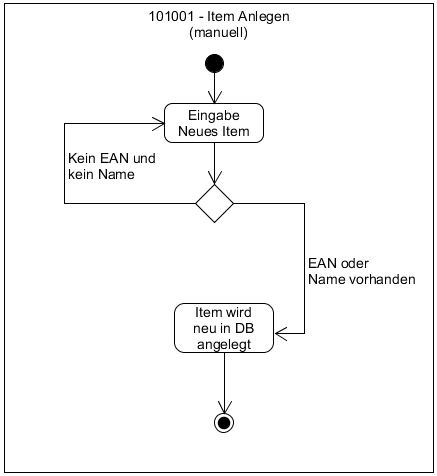
\includegraphics[scale=0.6]{pic/101001m}
	\caption{Aktivitätsdiagramm: Manuell Item anlegen}
\end{figure}

\subsubsection{Automatisches Anlegen eines Items}

Das automatische Anlegen eines Items ist in der App als Standard, für das Anlegen eines Items definiert. Sobald der User {\color{IndianRed}\texttt{Neues Item}} ausgewählt hat öffnet sich die Kamera. Der User muss nun nur noch den Barcode scannen (photographieren) und eine automatische Suche, im Internet, nach Metadaten zu diesem Barcode wird gestartet. Die gefundenen Metadaten werden dem User angezeigt und er kann diese nun bestätigen oder noch anpassen.

\begin{figure}[htbp]
	\centering
	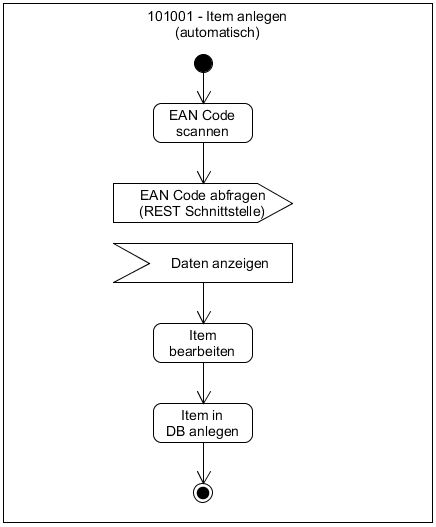
\includegraphics[scale=0.6]{pic/101001a}
	\caption{Aktivitätsdiagramm: Automatisch Item anlegen}
\end{figure}

\subsection{Bearbeiten eines Items}

[101002] Funktion: Item Bearbeiten\\

Ein vom User ausgewähltes Item, kann durch die Funktion {\color{IndianRed}\texttt{Bearbeiten}} manuell bearbeitet werden. Es gibt für den User keine Einschränkungen, jedes Datenelement kann angepasst werden.

\begin{figure}[htbp]
	\centering
	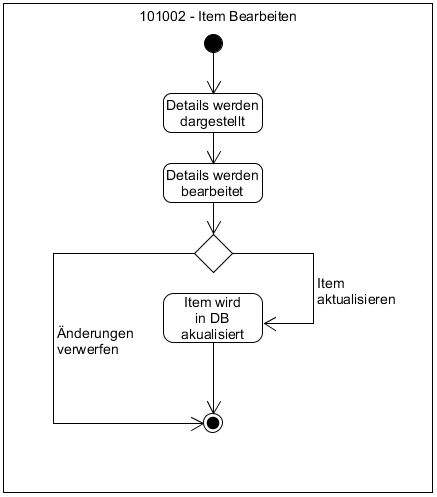
\includegraphics[scale=0.6]{pic/101002}
	\caption{Aktivitätsdiagramm: Item bearbeiten}
\end{figure}

\subsection{Löschen eines Items}

[101003] Funktion: Item löschen\\

Ein vom User ausgewähltes Item, wird komplett (mit all seinen Datenelementen) und unwiderruflich aus der Datenbank gelöscht. Zum Schutz vor unfreiwilligem Löschen, wird vor dem durchführen der Löschung der User nochmals aufgefordert den Löschvorgang zu bestätigen.

\begin{figure}[htbp]
	\centering
	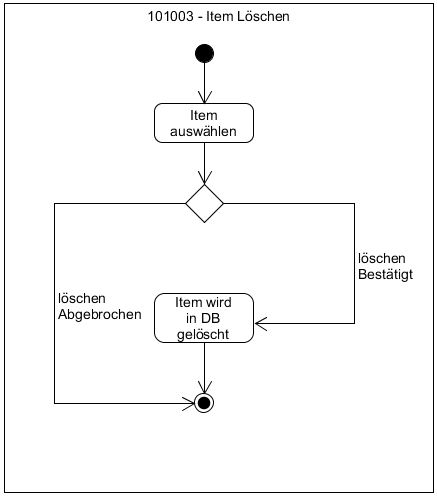
\includegraphics[scale=0.6]{pic/101003}
	\caption{Aktivitätsdiagramm: Item löschen}
\end{figure}

\subsection{Ausgabe der Items}

[102001] Funktion: Items anzeigen\\

Der User kann sich entweder die komplette Sammlung anzeigen lassen oder durch Eingabe eines oder mehreren Filterkriterien die angezeigt Auswahl einschränken. Jedes Kriterium, welches von einem Item gespeichert wird kann als Filter verwendet werden. Werden vom User mehrere Kriterien angegeben, werden diese mittels einer \emph{UND Verknüpfung} im Filter verwendet. 

\begin{figure}[htbp]
	\centering
	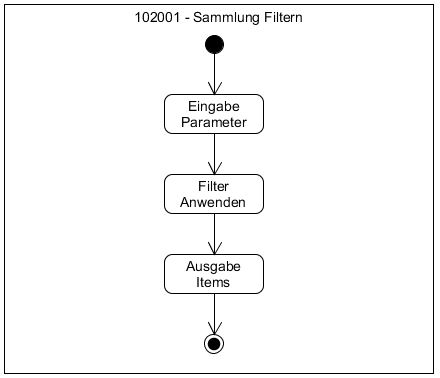
\includegraphics[scale=0.6]{pic/102001}
	\caption{Aktivitätsdiagramm: Sammlung anzeigen}
\end{figure}

\subsection{Verwalten verliehener Items}

[102002] Funktion: Items anzeigen\\

Der User kann ein Item als verliehen markieren. Wird ein Item so markiert, wird der User aufgefordert die leihende Person und das Datum einzugeben. Bei der Rückgabe des Items wird der Status von verliehen auf nicht verliehen geändert und das Item erscheint nun nicht mehr auf der Liste der verliehenen Gegenständen.\\
Eine History zeigt alle jemals verliehenen Gegenstände an.

\begin{figure}[htbp]
	\centering
	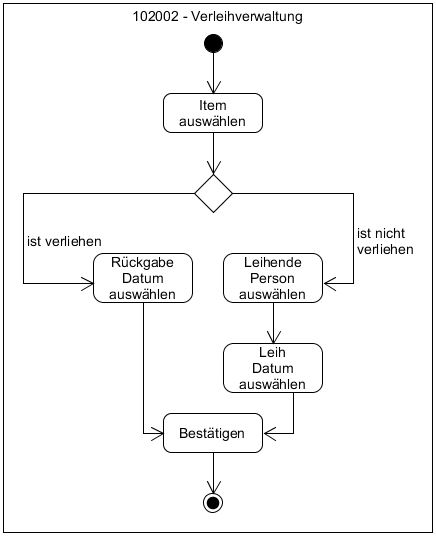
\includegraphics[scale=0.6]{pic/102002}
	\caption{Aktivitätsdiagramm: Verwalten verliehener Items}
\end{figure}

\subsection{Exportieren aller ausgewählter Items}

[102003] Funktion: Items anzeigen\\

Eine vollständige oder gefilterte Übersicht der Items einer Sammlung kann als CSV File exportiert werden. Das Export File wird auf der Speicherkarte des Smartphones gespeichert. Zusätzlich wird ein Mailprogramm geöffnet mittels welchem man das Export File versenden kann.

\begin{figure}[htbp]
	\centering
	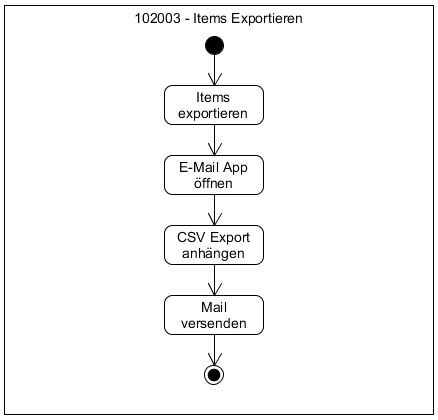
\includegraphics[scale=0.6]{pic/102003}
	\caption{Aktivitätsdiagramm: Export der Sammlung}
\end{figure}

\subsection{Datenbank Administration}

[102004] Funktion: Datenbank Administration\\

Die Datenbank Administration unterstützt folgende drei Aktionen für alle vorhanden Tables.

\begin{enumerate}
	\item Hinzufügen eines Eintrages
	\item Entfernen eines Eintrages
	\item Löschen der ausgewählten Tabelle
\end{enumerate}

\begin{figure}[htbp]
	\centering
	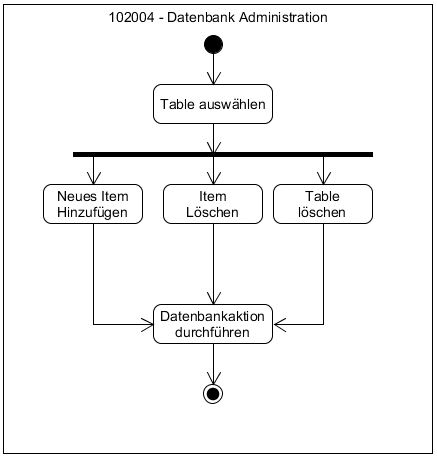
\includegraphics[scale=0.6]{pic/102004}
	\caption{Aktivitätsdiagramm: Datenbank Administration}
\end{figure}

\subsection{REST Schnittstelle zur Abfrage von Metadaten diverser Online Datenbanken}

[103001] Funktion: REST Schnittstelle zur Abfrage von Metadaten\\

Über eine REST Schnittstelle soll die App verschiedene Online Datenbanken abfragen. Anhand des gesendeten EAN Codes sollen eventuell vorhandene Metadaten zu den Items erfragt werden, so damit der User nicht alle Daten von Hand eingeben muss.

\subsection{Kamera als Barcodescanner}

[104001] Funktion: Kamera als Barcodescanner\\

Als weitere Eingabehilfe für den User soll die Kamera des Smartphones als EAN Scanner genutzt werden. Sollte diese den Barcode nicht erkennen können, kann der Barcode vom User manuell eingegeben werden.


\section{Datenbank}

Die Anforderungen der App an die Datenbank sind einfach und leicht überschaubar.

\subsection{Übersicht Datenbankfelder der Items}
\label{sec:Felder}

In der Tabelle \ref{tab:Datenbankfelder}  sind die Datenbankfelder für jedes Medium, Bücher, Filme und Spiele aufgeführt.

\begin{table} [htbp]
	\begin{center}
		\begin{tabular}{|l|l|l|l|}
			\rowcolor{black} {\color{white}\textbf{Allgemein}} & {\color{white}\textbf{Bücher}} & {\color{white}\textbf{Filme}} & {\color{white}\textbf{Spiele}} \\
			Barcode & Verlag & Studio & Entwickler\\ \hline
			\rowcolor{DarkSeaGreen} Titel & Auflage & Speichermedium & System \\ \hline			Medientyp & Autor& Regisseur & FSK \\ \hline
			\rowcolor{DarkSeaGreen} Genre & & FSK & \\ \hline
			Sprache & & Länge & \\ \hline
			\rowcolor{DarkSeaGreen} Erscheinungsjahr & & & \\ \hline
			Bewertung & & & \\ \hline
			\rowcolor{DarkSeaGreen} Lagerplatz & & & \\ \hline
			Verleihstatus & & & \\ \hline
			\rowcolor{DarkSeaGreen} Bemerkung & & & \\ \hline		
		\end{tabular}
	\caption{Datenbankfelder}
	\label{tab:Datenbankfelder}
	\end{center}
\end{table}

\newpage

\begin{landscape}
	\section{Übersicht Datenbank}
	\label{sec:UebersichtDB}
	\begin{figure}[htbp]
		\centering
		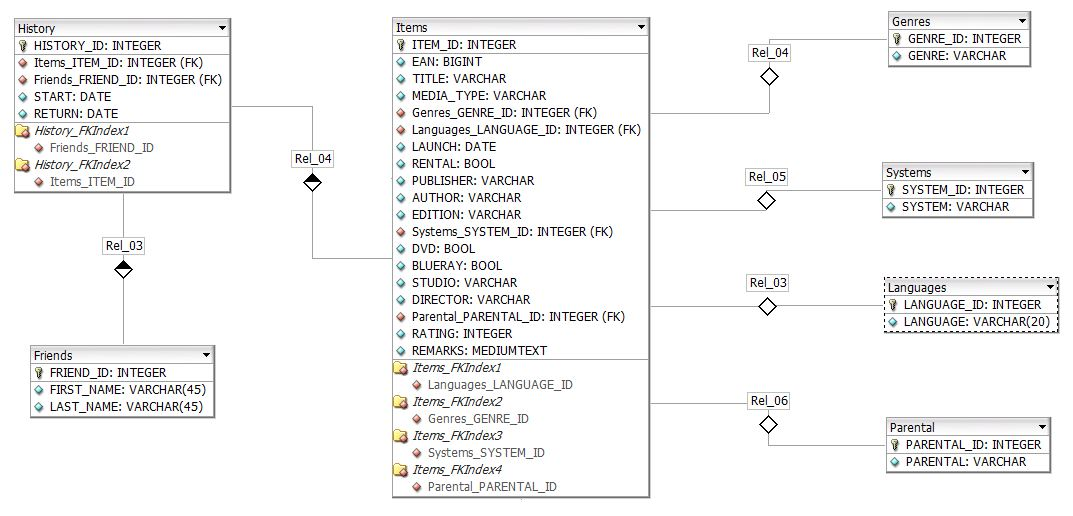
\includegraphics[scale=0.75]{pic/DbDesign}
		\caption{Überblick Datenbank}
	\end{figure}
\end{landscape}

\section{GUI}

Allgemein wird von der GUI erwartet, dass die App intuitiv bedienbar ist und fehlerfrei auf möglichst vielen Hardware Typen dargestellt werden kann. \\

Des weiteren ist die GUI  Design so angelegt, dass die App jederzeit übersichtlich ein Maximum an Informationen darstellen kann.

\subsection{Startseite}
\label{subsec:Startseite}

Die Startseite der App soll dem User ermöglichen auf alle wichtigen Funktionen direkt zuzugreifen. Deshalb besteht diese nur aus folgenden vier Buttons {\color{IndianRed}\texttt{Neues Item}}, {\color{IndianRed}\texttt{Sammlung}}, {\color{IndianRed}\texttt{Leihwesen}} und {\color{IndianRed}\texttt{Info}}.

\begin{figure}[htbp]
	\centering
	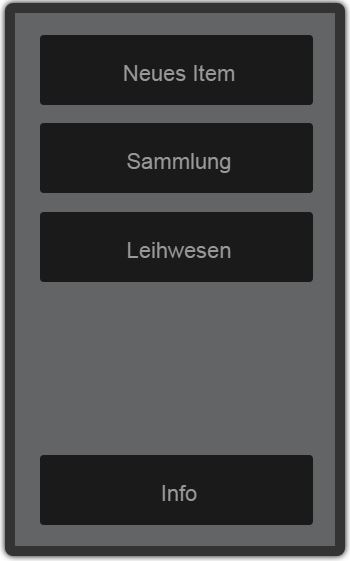
\includegraphics[scale=0.5]{pic/GUI/Main}
	\caption{Startseite}
\end{figure}

\subsection{Barcode Scannen}

Dieser Screen startet die eingebaute Kamera und wird automatisch angezeigt, wenn man ein neues Item anlegen will. Sollte das Item keinen Barcode besitzen, kann man von hier aus die Manuelle Eingabe erreichen. Eine zurück zur Startseite \ref{subsec:Startseite} ist ebenfalls möglich.

\begin{figure}[htbp]
	\centering
	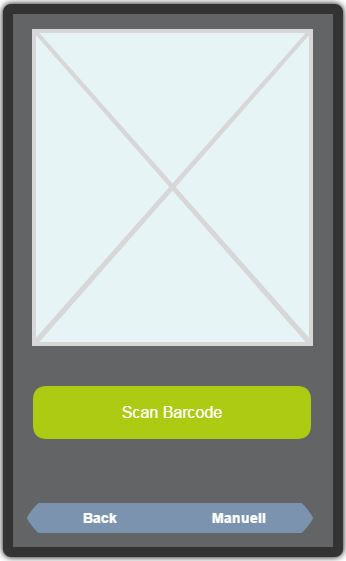
\includegraphics[scale=0.5]{pic/GUI/ScanBarcode}
	\caption{Barcode Scannen}
\end{figure}

\subsection{Manuell Anlegen / Item Bearbeiten}

Dieses Screenlayout wird sowohl für das manuelle Anlegen eines Items, als auch für das Bearbeiten eines vorhandenen Items genutzt.\\

Der einzige Unterschied besteht zwischen den beiden Aktionen darin, das dass beim manuellen Anlegen keine Datenelemente angezeigt werden. Während beim Bearbeiten eines Items, alle bisher gespeicherten Datenelemente angezeigt werden.

\begin{figure}[htbp]
	\centering
	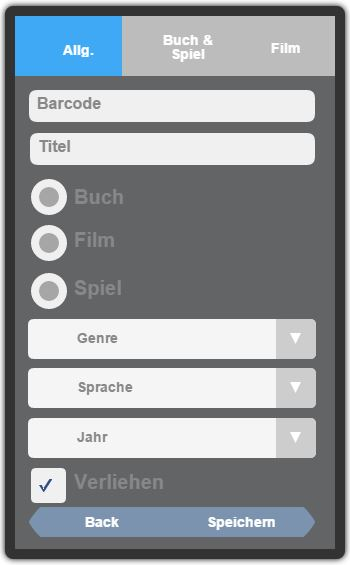
\includegraphics[scale=0.5]{pic/GUI/Manuell}
	\caption{Manuell Anlegen / Item Bearbeiten}
\end{figure}

\subsection{Detail Ansicht}

Hier werden dem User alle Datenelemente eines Items angezeigt. Ausserdem kann in dieser Ansicht das Item bearbeitet, verliehen oder gelöscht werden.

\begin{figure}[htbp]
	\centering
	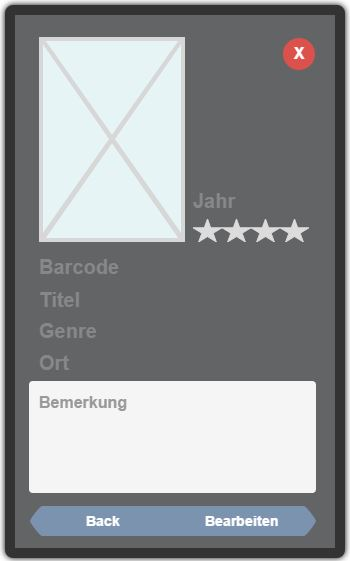
\includegraphics[scale=0.5]{pic/GUI/ItemAnsicht}
	\caption{Detail Ansicht}
\end{figure}

\subsection{Sicherheitsfrage Item Löschen}

Wenn der User ein Item aus der Datenbank (Sammlung) löschen will. Erscheint immer bevor der Löschvorgang gestartet wird folgende Sicherheitsfrage.

\begin{figure}[htbp]
	\centering
	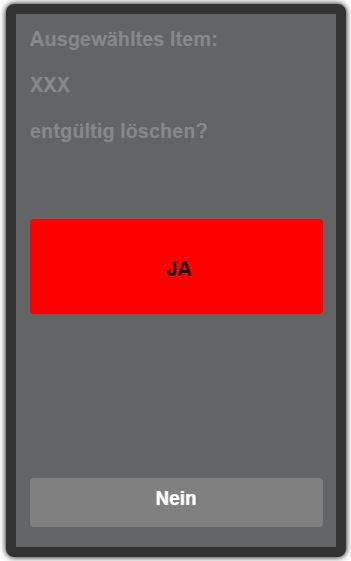
\includegraphics[scale=0.5]{pic/GUI/DeleteItem}
	\caption{Sicherheitsfrage}
	\end{figure}
	
\subsection{Item verleihen}

Wird ein Item als verliehen markiert, erscheint eine erweiterbare Liste mit Personen. Aus dieser Liste wählt der User nun die Person aus, welche das Item geliehen hat. Ist die Person noch nicht in der Liste, kann der User diese in die Liste eintragen.

\begin{figure}[htbp]
	\centering
	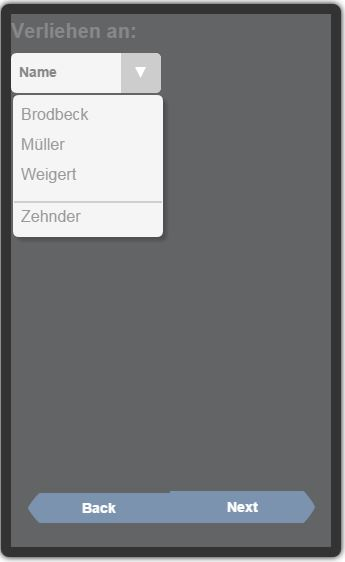
\includegraphics[scale=0.5]{pic/GUI/VerliehenAn}
	\caption{Item verleihen}
\end{figure}

\section{Allgemeines}

\subsection{Dokumentation der Anforderungen}

Die Anforderungen werden um Mehrdeutigkeit und offene Definitionen zu vermeiden nach folgenden Modellen der Anforderungsanalyse

\begin{itemize}
	\item Natürliche Sprache
	\item Aktivitätsdiagramm
	\item Use Case
\end{itemize}

dokumentiert. \\
Bei komplexeren Anforderungen, welche durch die verwendeten Modelle nicht eindeutig dokumentiert werden können, werden zur Spezifizierung noch weitere UML Modelle eingesetzt. \\

Diese weiteren Modelle wird aus den Notationen von UML 2.3 so ausgewählt, dass die Anforderung Eindeutig beschrieben werden kann.

\subsubsection{Natürliche Sprache}

Um die Mehrdeutigkeit und den möglichen Interpretationsspielraum der natürlichen Sprache zu minimieren, muss die Dokumentation der Anforderung in natürlicher Sprache folgenden Regeln genügen.

\begin{itemize}
	\item Anforderungen immer anhand der Prozesse erklären.
	\item Jeder Prozess einer Anforderung muss eindeutig beschrieben sein.
	\item Substantive, welche zur Anforderungs- oder Prozess Beschreibung eingesetzt werden, müssen über den Bezug für den Leser eindeutig sein.
	\item Bei Mengen und Häufigkeiten nur folgende Quantoren benutzen.
	\begin{itemize}
		\item immer / nie
		\item jeder / kein
		\item alle / irgendein(er) / nichts
	\end{itemize}
	\item Bedingungen immer vollständig dokumentieren.
	\item Nur den sprachlichen Aktiv verwenden.
\end{itemize}

\subsection{Systematik der Anforderungen}

Jede Anforderung erhält eine eindeutige sechsstellige Anforderungsnummer. Diese leitet sich aus folgenden drei Bestandteilen ab.

\begin{enumerate}
	\item Art der Anforderung (Funktionelle, Datenbank, GUI, Sonstige)
	\item Priorität (1 bis 4)
	\item Laufende eindeutige Nummer
\end{enumerate} 

\subsubsection{Art der Anforderung}

Zur Gliederung wird eine zweistellige Nummer verwendet.

\begin{table} [htbp]
	\begin{tabular}{r|l}
		\textbf{Nr.} & \textbf{Art der Anforderung} \\ \hline
		10 & Anforderung an die Funktion der App \\
		\rowcolor{DarkSeaGreen} 20 & Anforderung an die Datenbank \\
		30 & Anforderung an das GUI \\
		\rowcolor{DarkSeaGreen} 40 & Sonstige Anforderungen
	\end{tabular}
\end{table}

\subsubsection{Priorität der Anforderung}

Die Priorität der Anforderung wird in Ziffern 1 (höchste) bis 4 (niedrigste) definiert.

\begin{enumerate}
	\item Grundlage (bzw. absolutes Muss)
	\item Muss für Grundlegende Funktionen der App
	\item Steigerung der Usability für den Nutzer
	\item Wäre eine tolle zusätzliche Funktion.
\end{enumerate}

\subsubsection{Beispiel: Nummerierung und Bezeichnung der Anforderung}

Die Anforderung  \glqq\emph{Datenbank Design}\grqq \ hat folgende Anforderungsnummer (ID):\\

	\begin{tabular}{c|c|c}
		\textbf{Art} & \textbf{Prio} & \textbf{lfd. Nummer} \\
		\emph{2-stellig} & \emph{1-stellig} & \emph{3-stellig} \\ \hline
		20 & 1 & 001 \\
	\end{tabular}\\

Die komplette Bezeichnung der Anforderung würde wie folgt aussehen. \\

[201001] Datenbank: Design

\subsection{Systemanforderungen}

Die App wurde für ein Samsung Galaxy S5 mit Android 5.0 entwickelt. Aufgrund der verwendeten Android Layouts,
 sollte die App allerdings ohne Probleme auf allen Android Smartphones und Tablets mit mindestens Android 5.0 
 funktionieren.
\chapter{Konzept}

\section{Datenbank}

Die Anforderungen der App an die Datenbank sind einfach und leicht überschaubar.

\subsection{Übersicht Datenbankfelder der Items}
\label{sec:Felder}

In der Tabelle \ref{tab:Datenbankfelder}  sind die Datenbankfelder für jedes Medium, Bücher, Filme und Spiele aufgeführt.

\begin{table} [htbp]
	\begin{center}
		\begin{tabular}{|l|l|l|l|}
			\rowcolor{black} {\color{white}\textbf{Allgemein}} & {\color{white}\textbf{Bücher}} & {\color{white}\textbf{Filme}} & {\color{white}\textbf{Spiele}} \\
			Barcode & Verlag & Studio & Entwickler\\ \hline
			\rowcolor{DarkSeaGreen} Titel & Auflage & Speichermedium & System \\ \hline			Medientyp & Autor& Regisseur & FSK \\ \hline
			\rowcolor{DarkSeaGreen} Genre & & FSK & \\ \hline
			Sprache & & Länge & \\ \hline
			\rowcolor{DarkSeaGreen} Erscheinungsjahr & & & \\ \hline
			Bewertung & & & \\ \hline
			\rowcolor{DarkSeaGreen} Lagerplatz & & & \\ \hline
			Verleihstatus & & & \\ \hline
			\rowcolor{DarkSeaGreen} Bemerkung & & & \\ \hline		
		\end{tabular}
	\caption{Datenbankfelder}
	\label{tab:Datenbankfelder}
	\end{center}
\end{table}

\newpage

\begin{landscape}
	\section{Übersicht Datenbank}
	\label{sec:UebersichtDB}
	\begin{figure}[htbp]
		\centering
		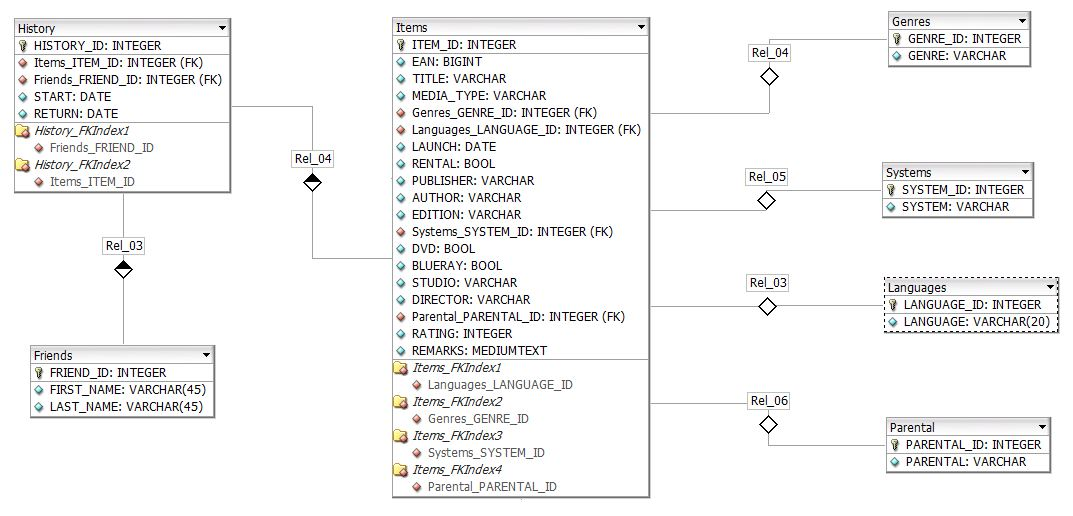
\includegraphics[scale=0.75]{pic/DbDesign}
		\caption{Überblick Datenbank}
	\end{figure}
\end{landscape}
\chapter{Umsetzung}
\chapter{Testing}

% --------------------------------------ANHANG--------------------------------------------

% Die Inhalte des Anhangs werden analog zu den Kapiteln implementiert; über die Datei
% Anhang.tex

\begin{appendix}
%	\clearpage
%	\pagenumbering{Roman}
%	\renewcommand{\thesection}{\arabic{section}}
	\chapter{Anhang}

\section{Konventionen}

Für die Beschreibung von Eingaben oder Beschriftungen in der App wird folgendes Format benutzt. \\
{\color{IndianRed}\texttt{Beispiel einer Eingabe durch den User oder Beschriftung in der App.}}

\section{Verwendete Tools \& Software}

\subsection{Dokumentation \& Präsentation}

Alle Dokumente und Präsentationen wurden in \LaTeX \ geschrieben. Dazu wurde \href{http://texstudio.sourceforge.net}{TeXstudio} in der Version 2.10.4 genutzt. 

\subsection{Programmierung}

Die App wurde im \href{https://developer.android.com/studio/index.html}{Android Studio} 1.5.1 von Google erstellt.\\
Zusätzlich wurde für den CSV Export die Library \href{http://opencsv.sourceforge.net/}{Opencsv} in der Version 3.7 genutzt.

\subsection{Code und Versionsverwaltung}

Für die Versionsverwaltung aller Dokumente und des Programmcode wurde auf GitHub ein \href{https://github.com/MWeigert/Collector}{Repository} eingerichtet.

\subsection{Datenbank}

Für die Erstellung des Datenbank Design wurde der \href{http://fabforce.net/dbdesigner4/}{DB Designer 4} von fabFORCE.net verwendet.

\subsection{GUI}

Für die Funktion und das Design der GUI wurde das Webtool \href{https://www.fluidui.com}{Fluid} genutzt.

\subsection{UML}

Sämtliche UML wurden mit dem freien Tool \href{http://www.umlet.com}{Umlet} erstellt.  

\section{Design Entscheidungen}

\begin{tabular}{|c|l|c|l|}
	\rowcolor{black} {\color{white}\textbf{ID}} & {\color{white}\textbf{Datum}} & {\color{white}\textbf{Autor}} & {\color{white}\textbf{Bemerkung}} \\
	001 & 12.03.16 & M. Weigert & Hauptsprache für App wird Englisch \\ \hline
	\rowcolor{DarkSeaGreen} 002 & 12.03.16 & M. Weigert & Es wird auf jeden Zurück/Back Button verzichtet. \\ \hline
	003 & 25.03.16 & M. Weigert & Extra Tabelle Parental um internationale Jugendfreigaben zu managen. \\ \hline
	\rowcolor{DarkSeaGreen} 004 & 09.04.16 & M. Weigert & Verzicht auf die Tabelle Parental um die App nicht unötig zu komplizieren. \\ \hline
\end{tabular}
	\bibliography{bib/mybib.bib}
	\bibliographystyle{unsrt}
\end{appendix}

% ----------------------------------------------------------------------------------------

\end{document}
